% Submission draft. The author's affiliation and corresponding-author contact remain to be supplied.
% EAB title and layout follow the supplied manuscript examples.
\documentclass[conference]{IEEEtran}
\usepackage[T1]{fontenc}
\usepackage{amsmath,amssymb,booktabs,multirow,xcolor,url,tabularx,array}
\usepackage{graphicx}
\usepackage[hidelinks]{hyperref}
\title{[Experiment, Analysis, and Benchmark] Evaluating Language Models and Subspace Methods for Explaining Known Tabular Outliers}
\author{\IEEEauthorblockN{Lili Guan}\\
\IEEEauthorblockA{ORCID: \url{https://orcid.org/0000-0002-4464-9384}}}
\begin{document}
\bstctlcite{IEEEcompactreferences}
\maketitle

\begin{abstract}
Explaining a flagged table row requires deciding which fields jointly distinguish it from normal data. Row labels and injected edits do not determine this explanation: a modified field can be ordinary alone, and several irreducible combinations can be valid. We present a benchmark that completely enumerates population-minimal support explanations, separates them from rule and edit targets, and audits the evidence available in finite references. A unified comparison gives three local language models and subspace methods the same candidate information and budget, with fixed structured output for the models. It also includes direct enumeration of sample-minimal explanations. On 96 paired targets, Qwen reaches exact recovery of 0.385 and Gower-LOF 0.646; the enumeration baseline reveals a separate gap between candidate coverage and first-choice ranking. Complete-population, new-rule, invoice, and public expert-decision workloads expose different failure modes. Invoices show how duplicate-sensitive density ratios compete across discrete projections: treating distinct-coordinate neighborhoods raises LOF recovery from 0.000 to 0.229, while changing the numerical floor does not improve it. Public correction records provide a separate inspection target. These results show how label semantics, available evidence, and method configuration determine anomaly-explanation comparisons.
\end{abstract}
\begin{IEEEkeywords}
data quality, anomaly explanation, feature subspaces, large language models, benchmark evaluation
\end{IEEEkeywords}

\section{Introduction}
Investigating a data-quality alert requires choosing fields to inspect. A value can be ordinary alone and unusual in combination with other attributes. In \emph{known-outlier explanation}, a method receives a flagged row, its schema, and finite normal references, then returns ranked field subsets. The upstream detector score and the target's clean counterpart are unavailable~\cite{li2024xadsurvey}. The evaluation must specify what makes one of those subsets a correct explanation.

\textbf{One invoice, different targets.} Consider net $25$, tax $1$, and gross $14$ (Figure~\ref{fig:intro-support}). The finite clean domain permits net values $\{10,15,20,25\}$, tax values $0$--$4$, and gross $=\text{net}+\text{tax}$. The recorded edit changes gross. Yet gross 14 also occurs in the normal triple $(10,4,14)$, so the edited singleton does not exclude normal data. Both \{net, gross\} and \{tax, gross\} are minimal exclusions. Their union excludes normal data too, but contains a redundant field. Recovering the edit, a sufficient combination, and a minimal explanation therefore produces different answers for the same row.

\begin{figure}[t]
\centering
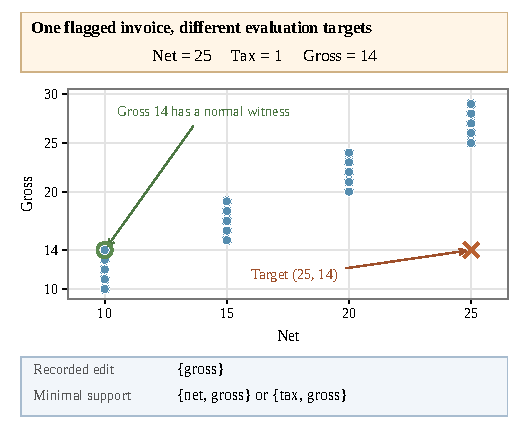
\includegraphics[width=\columnwidth]{figures/figure_intro_support_semantics.pdf}
\caption{The recorded invoice used throughout the paper. Blue points are all 20 clean net--gross pairs; the cross is the target. Gross 14 has a normal witness, whereas the pair $(25,14)$ has none. The recorded edited field and the two minimal support explanations are different evaluation targets.}
\label{fig:intro-support}
\end{figure}

\textbf{Why compare language models?} A prompt can describe mixed field types, serialize examples, and request candidate subsets without fitting a separate model to every schema. LLM-based data-quality systems such as ZeroED and ZeroEC generate criteria, labels, or correction rules from context~\cite{ni2025zeroed,wu2025zeroec}. Table-anomaly and cleaning benchmarks similarly motivate evaluating this interface~\cite{choudhury2025tabard,gu2025radar,li2025autodcworkflow}. Here, three fixed local models must infer useful combinations from the supplied rows. Opaque or neutral names restrict the main comparison to that evidence; the experiment does not establish performance for larger models, tool-using systems, or domain-rich prompts.

\textbf{The evaluation problem.} Relevant-subspace evaluation already allows multiple correct subsets and exact set matching~\cite{myrtakis2021comparative}. The unresolved issue addressed here is how to define \emph{all} minimal explanations of a population, distinguish those labels from an edit history, and assess methods that see only a sample. A projection absent from the references may occur elsewhere in the normal population. Conversely, a model may return a supported or redundant set even when every normal row is visible. Candidate size information and output requirements can further change a method comparison.

\textbf{Our approach.} We enumerate complete finite clean populations and retain every inclusion-minimal support exclusion, with separate rule and provenance labels. The original 864-case study supplies 38 test templates and exposes evidence ambiguity. We then compare methods under one frozen core task: identical targets, references, candidate-size information, and four-candidate budgets; the LLMs use a minimal JSON schema. A sample-minimal enumeration baseline directly checks the visible support relation. The same configuration is applied to new rule compositions, invoice constraints, and an independent public expert decision table. Figure~\ref{fig:framework} connects these inputs, candidate generators, and evaluation targets.

The study follows three questions. \textbf{RQ1: Labels.} How do population support, rules, and recorded changes alter explanation evaluation? \textbf{RQ2: Evidence and configuration.} How do finite references, candidate priors, and output contracts affect comparisons under a common core task? \textbf{RQ3: Scoring mechanisms.} Why can a subspace ranker's performance reverse across workloads, and which implementation choices contribute?

Our contributions are:
\begin{itemize}
\item \textbf{Complete population-minimal labels and evidence audits.} We distinguish support, rule, mechanism, and edit targets. Sample-minimal families differ from population labels in 862 of 864 original cases; deterministic proxies change the support and rule labels in 211 cases.
\item \textbf{A unified comparison with a direct support baseline.} Shared candidate information and fixed structured output enter the same experiments. Sample enumeration separates finding plausible candidates from ranking them, while repeated references and complete populations diagnose available evidence.
\item \textbf{A mechanism analysis of discrete subspace ranking.} Matched invoice experiments isolate numerical floors, boundary ties, and duplicate handling. Public corrections and expert decisions clarify which conclusions transfer under unchanged explanation semantics and which concern a different target.
\end{itemize}

\begin{figure*}[t]
\centering
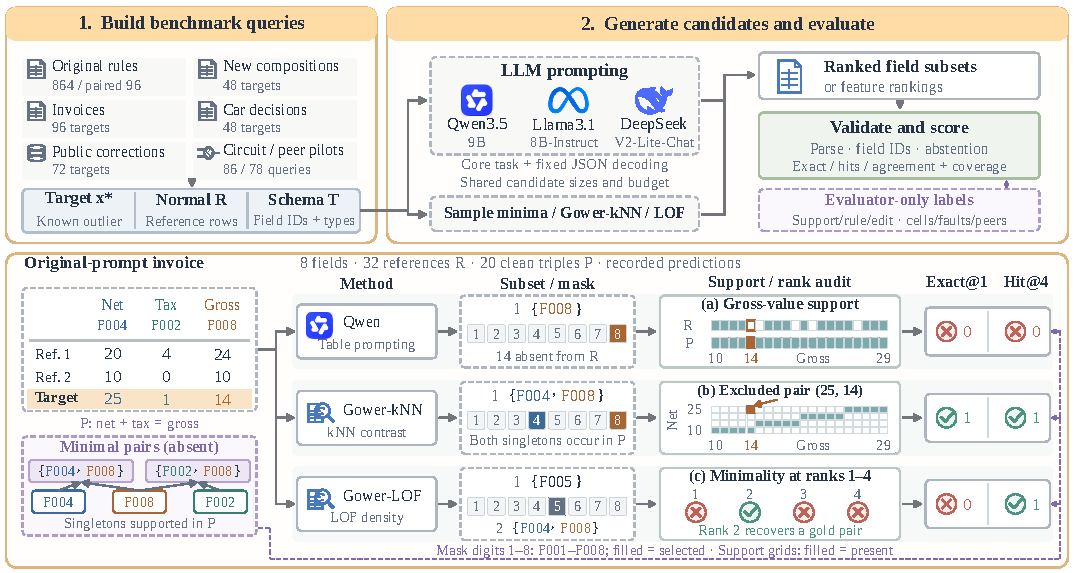
\includegraphics[width=\textwidth]{figures/figure2_overall_framework.pdf}
\caption{Evaluation framework and recorded invoice \texttt{constraint\_tax\_total\_000}. The overview shows the unified core task; auxiliary tracks retain their own configurations and labels. The lower trace preserves outputs from the original prompt, illustrating why candidate generation and support verification differ. It displays three of eight fields and two of 32 references. Gross 14 is absent from $R$ but present in the 20-triple population $P$; the net--gross pair is excluded; LOF's second candidate is minimal. Purple paths carry evaluator-only information.}
\label{fig:framework}
\end{figure*}

\section{Task and Label Semantics}

Given schema $T$ with fields $F=\{f_1,\ldots,f_d\}$, known outlier $x^*$, and normal references $R$, a method returns ranked subsets
\[
\widehat{\mathcal E}(x^*,R,T)=(S_1,\ldots,S_K),\qquad S_k\subseteq F,
\]
optionally with evidence, confidence, or abstention.

Let $P_X$ denote the clean population and $\pi_S$ the projection onto $S$. A subset is \emph{support-sufficient} when $\pi_S(x^*)$ has no match in $P_X$. It is \emph{rule-sufficient} when every full domain assignment matching $x^*$ on $S$ satisfies the anomaly predicate. A sufficient subset is inclusion-minimal when no proper subset is sufficient. We retain the complete minimal families $\mathcal S_{\mathrm{support}}^{\min}$ and $\mathcal S_{\mathrm{rule}}^{\min}$; inclusion-minimal sets can differ in size. Separate provenance labels record directly edited fields $M_{\mathrm{direct}}$, all value changes $M_{\mathrm{value}}$ including propagation, and fields capable of affecting the anomaly rule $M_{\mathrm{rule}}$.

\textbf{When support and rule labels coincide.} Let $\mathcal D$ be the disclosed Cartesian domain and $A$ the anomaly predicate. If $P_X=\{x\in\mathcal D:\neg A(x)\}$, absence of a clean completion is equivalent to every completion satisfying $A$. The two minimal families then coincide. Additional clean-population constraints can break this equivalence: a deterministic proxy can exclude clean completions without appearing in $A$. Section V-A gives an observed example.

For $A(f_1)\lor B(f_2)$ with both terms true, either singleton can be minimal, whereas their union is redundant. Our primary label is population-minimal descriptive support; Table~\ref{tab:semantics} separates it from unobserved edit provenance.

A population-absent projection is absent from $R$, but sampling can create additional absences. We keep population labels fixed and audit sample-minimal alternatives separately.

\textbf{Checking an explanation.} For a clean row $r$, let $D(r)=\{f_j:r_j\ne x^*_j\}$ contain the fields on which it differs from the target. Then support sufficiency is equivalent to
\[
  S\cap D(r)\ne\varnothing\quad\text{for every }r\in P_X.
\]
Each normal row must therefore be distinguished by at least one selected field. To check minimality, remove each field $f$ from $S$ in turn. A minimal set has a normal witness matching $x^*$ on $S\setminus\{f\}$ for every such removal. These witnesses show why every selected field is necessary. Checking single-field removals suffices because absence is preserved when more fields are added. Replacing $P_X$ by $R$ gives the sample criterion, which has fewer rows to distinguish and can admit additional explanations.

For the invoice in Figure~\ref{fig:framework}, gross 14 occurs with net 10 and tax 4, and net 25 occurs with other gross values. Both singletons thus have normal witnesses, whereas the pair $(25,14)$ has none. A large candidate containing this pair is sufficient but need not be minimal. This distinction also explains why a feature ranking alone cannot certify an explanation: its prefix length and the joint support of the selected values determine whether the candidate meets the task definition.

\begin{table}[t]
\centering\footnotesize
\caption{Label semantics and identification from an unpaired query with finite normal references and no hidden generator.}
\setlength{\tabcolsep}{3pt}
\renewcommand{\arraystretch}{1.12}
\begin{tabularx}{\columnwidth}{|l|>{\raggedright\arraybackslash}X|>{\raggedright\arraybackslash}p{1.65cm}|}
\hline
Label & Meaning and inferability & Use \\
\hline
Support & Minimal absent projections; finite references need not identify them & Primary \\
Rule & Minimal subsets forcing anomaly; hidden predicate required & Alternative \\
Mechanism & Fields affecting anomaly; hidden rule required & Relevance \\
Direct edit & Recorded edits; hidden intervention history required & Provenance \\
Value change & Changes including propagation; paired clean row required & Provenance \\
Corrected field & Published dirty/clean difference; source convention required & Inspection \\
Peer agreement & Overlap with other model selections; no field truth & Agreement \\
\hline
\end{tabularx}
\renewcommand{\arraystretch}{1.0}
\label{tab:semantics}
\end{table}



\section{Benchmark Construction}
\subsection{Procedural support benchmark}

Each of three seeds generates 40 templates with 12 cases each, split into eight training, eight development, and 24 test templates. The combined 864 test cases cover 38 templates. Splits are disjoint within a seed, but development/test unions overlap across seeds. This version was reevaluated after inspecting earlier results. Bootstrap and multiplicity correction describe repeated evidence on 38 templates; they cannot remove that selection bias. The new-composition validation freezes methods before generating different rules.

Eight families cover numeric marginals, categorical rarity, pairs, conditional groups, multiple valid sets, edit/mechanism differences, relational comparisons, and higher-order logic. Each seed tests three of five templates per family; pooled family summaries involve four or five templates and remain descriptive.

Cases contain 6/12/24 fields and 8/16/32 references, with finite numeric, ordinal, binary, categorical, date-like, and identifier-like domains. Marginal factors are balanced; joint cells are not. Six nuisance profiles cover independent noise, a 64-category distractor, noisy and deterministic proxies, a pre-edit frozen proxy, and independent categorical missingness. Dates and identifiers are distractors. Complete profiles and joint case/template counts are in the artifact.

The generator enumerates clean/anomalous role assignments, samples a hidden clean row and target, binds roles to random IDs, and adds distractors and references. Sufficient subsets are enumerated with deterministic proxy constraints, then nonminimal sets are removed. Independent distractors are marginalized. Changing individual roles checks rule relevance; direct and propagated changes are recorded separately. Rule IDs, logic, clean rows, and labels are withheld.

An independent seeded permutation then determines schema, target, and reference column order, preserving values, labels, and field-name bindings. Identity permutations are allowed. Half the cases expose random neutral names. Separate display seeds prevent the role-binding prefix from becoming a fixed cue.




The primary paired panel consists of all 96 first-split test targets with 32 references, four per template. Its selection is independent of method outputs. This panel supports a controlled comparison on 24 original templates, not an independent replacement for the original test distribution.

\subsection{Standards-derived invoice constraints}

An independent finite-domain workload instantiates four Peppol billing relations~\cite{peppol2026billing}: line net equals quantity times unit price plus charges minus allowances (R120, base quantity one); document net equals summed line nets plus charges minus allowances (BR-CO-13); gross equals net plus tax (BR-CO-15); and amount due equals gross minus paid plus rounding (BR-CO-16). These are synthetic integer amounts, not collected invoices or a full conformance test.

We enumerate each normal relation, yielding 144, 144, 20, and 48 structured rows. One structured field of a clean row is changed to another value in its own clean marginal. We retain 24 distinct invalid targets per relation before model inference. Each of the 96 queries has eight opaque fields, independent categorical distractors, 32 sampled clean references, and independent display order. Complete population enumeration gives all minimal support alternatives, marginalizing independent distractors. The anomaly predicate is the complement of the normal relation, so support and rule labels coincide. Direct edits remain separate. The original prompt is retained as a diagnostic; the unified comparison uses the core configuration of Section IV. Both Gower methods search all 255 nonempty subsets. Scores average targets within each relation and the four relations equally; they are descriptive for these fixed relations.



\subsection{New compositions and complete evidence}

We freeze the three checkpoints, original full prompt, parser, and decoding protocol before generating 48 targets from 12 new Boolean compositions. Each composition has four to six essential coordinates in six visible binary fields; the original generator's rules have at most three. The new rules include parity, disjoint conjunctions, conditional parity, a multiplexer, count balance, and majority-output consistency. Their complete 64-row truth tables are distinct. Four invalid targets per rule are selected with a fixed seed before inference. Both Gower methods search all 63 nonempty subsets, with the same four-answer budget as the models.

Each target receives an independent 32-row sample with replacement. The first two targets per rule, fixed before inference, additionally receive two independent samples and the complete normal population. This gives 24 matched targets under three draws and complete evidence, or 120 inputs per method in total. Complete evidence contains every normal six-field tuple, including all nuisance combinations, and the prompt explicitly identifies it as complete. This condition changes evidence coverage and the completeness declaration together. The rules are newly designed after review, rather than externally curated blind tasks; model and protocol choices are not adjusted to their results.

We average targets within each new rule and the 12 rules equally. Prespecified strata use minimum truth size (1--2, 3, 4--6), number of minimal alternatives (1, 2--4, 5 or more), and extra sample minima (0, 1--3, 4 or more). Repeated samples hold target, schema, display order, and population labels fixed. They measure sampling sensitivity without treating repeated observations as independent tasks.


The unified configuration is fixed before its new generations on these existing queries. We retain the original full-prompt results as diagnostics; the joint rerun does not make this previously examined workload a fresh blind test.

\subsection{Independent expert decision table}
UCI Car Evaluation is derived from an expert decision model and completely covers its six-attribute categorical domain~\cite{bohanec1988car}. We verify that the 1,728 distinct rows equal the Cartesian product of the published domains. The 518 configurations labeled acceptable, good, or very good define $P_X$; an unacceptable configuration is the flagged target. Exhaustive projection checks produce the same population-minimal support labels as in Section II. This supplies an independent source of normal constraints, with no injected edit serving as explanation truth.

Before inference, a fixed seed selects 12 unacceptable targets per buying-price category, for 48 targets. Each query receives 32 acceptable references sampled without replacement. Random opaque field IDs and independently shuffled display order preserve the categorical values. The price stratum is used for selection only; source labels, decision rules, and full populations are hidden. All 63 nonempty subsets are eligible. Results describe this one expert decision system; its configurations are not observed anomaly incidents, and opaque IDs do not exclude pretraining exposure.

\subsection{Auxiliary targets}
\textbf{Public corrections.} We retain 72 queries from the Flights, Beers, and Rayyan dirty/clean pairs distributed with Raha and Baran~\cite{mahdavi2019raha,mahdavi2020baran}. Each source contributes 24 targets: eight with one, two, or at least three recorded corrections, chosen before the original predictions. Methods receive 32 corrected reference rows excluding held-out targets; Flights also excludes other records of the same flight. Raw strings and source row identities are preserved; record-index fields are removed. The hidden corrected counterpart supplies acceptable singleton inspection targets, including source-specific formatting changes. These labels do not enumerate minimal support explanations.

\textbf{Circuits and peer agreement.} Sixteen table pairs from four gate-negation circuits yield 64 targets and 86 focus-output queries, with 16 references each. Their fault input sets contain 1--12 fields; 47 exceed three. The artifact verifies changed-output alignment over 66,834 anomalous rows~\cite{antwarg2024groundtruth}. A separate five-model pilot covers 70 ADBench queries and eight UCI Lymphography queries~\cite{han2022adbench,zwitter1988lymphography}. UCI uses two source-class-1 normal rows, whereas ADBench uses its binary labels and 142 normal rows. Circuit fault recovery and peer agreement retain their own denominators and are never pooled with support accuracy.

\section{Evaluation Protocol}
\subsection{Unified core configuration}
The primary comparison includes Qwen3.5-9B, DeepSeek-V2-Lite-Chat, Llama-3.1-8B-Instruct, sample-minimal enumeration (SME), Gower-kNN, and Gower-LOF. All receive the same target, schema, normal rows, and field order. The LLMs return only ranked feature subsets and an abstention flag. They are explicitly told the same size cap used by search: three fields on the paired panel, six on new rules and Car decisions, and eight on invoices. Every method has a budget of four distinct nonempty subsets. No field identities or hidden labels accompany the size information.

The three checkpoints use the existing shared loader and chat templates, greedy batch-one decoding, a 16,384-token input limit without truncation, and 512 output tokens. A fixed JSON-schema token filter enforces the core object, legal IDs, four candidates, and the relevant size cap~\cite{lmfe2026}. The original parser rejects repeated IDs; repeated candidate sets collapse in their existing order. An oversized or empty set invalidates an answer, without truncating or reranking fields. Abstention suppresses attached candidates. Invalid, missing, input-rejected, and abstained queries remain recovery failures.

This configuration is frozen before 1,080 new model queries: 360 per checkpoint, covering the paired panel, all 120 new-rule evidence conditions, 96 invoices, and 48 Car decisions. It follows inspection of earlier experiments and is not a preregistered confirmation. The comparison evaluates these checkpoints, prompts, and decoding rules together. Auxiliary task classification, mechanism descriptions, evidence sentences, and confidence values are excluded from the core contract.

\subsection{Direct sample-minimal enumeration}
SME enumerates every nonempty field set within the shared cap using only the target and visible reference rows. A set is retained when the target projection is absent and every single-field removal restores a match. Candidates are sorted by cardinality and then the canonical feature-ID tuple; the first four are returned. This rule is fixed before scoring and uses neither population labels nor learned field relevance. Canonical IDs prevent display order from changing ties, but are not a claim of an optimal ranking policy.

We report the full candidate family's size and population-label retention as diagnostics in addition to top-four recovery. These quantities distinguish failure to expose a population minimum from failure to rank it. With complete normal evidence and a full candidate space, SME must return valid population minima whenever the target is outside that population. This is a correctness reference implied by the definition. With finite references, additional absences can create small spurious candidates that precede valid population explanations.

\subsection{Statistical rankers and original adapters}
\textbf{Gower rankers.} Gower distance averages reference-range-scaled differences for numeric, ordinal, and date-like fields and mismatch distances for categorical, binary, and identifier fields~\cite{gower1971similarity}. Missing-value mismatches score one. Exhaustive search uses the same candidate caps as the LLMs and SME. Gower-kNN ranks the target's three-neighbor mean distance relative to the median and dispersion of reference leave-one-out distances. Gower-LOF uses reference-only local reachability densities~\cite{breunig2000lof}. The target never enters the fitted reference graph. Score ties are resolved by subset size and canonical IDs. The existing ranker predictions are reproduced exactly on all 312 previously evaluated query conditions per method.

\textbf{Original diagnostic suite.} The 864-case comparison retains its original full LLM contract and unequal size prior: Gower knew that all population minima had at most three fields, while the model prompt did not. Table~\ref{tab:original} is therefore secondary to the unified comparison. Controls include all fields, the first three display positions, a univariate rarity/deviation ranking, and random subsets whose size distribution is estimated from training labels over 100 random seeds. SME is added under the same three-field cap.

SOD, COP, and M\textsuperscript{2}OE use legal-domain scaling, one-hot categorical encoding, and explicit missing coordinates~\cite{kriegel2009sod,kriegel2012cop,angiulli2024m2oe}. Their outputs are task adaptations: SOD selects a low-variance subspace, COP maps local-PCA errors to fields, and M\textsuperscript{2}OE supplies both field choices and repair masks. M\textsuperscript{2}OE's unordered choices use a separate three-choice endpoint. The paper-guided RLAX adaptation uses a reference-distance PPO reward with 256 interactions and four epochs, with 1,024/4,096-interaction development diagnostics~\cite{amirato2026rlax}. Beam retains 100 pairs before expanding to triples; a matching exhaustive pair/triple search isolates pruning~\cite{myrtakis2021comparative}. We make no convergence or speed claims for these adapters.

\subsection{Metrics, aggregation, and uncertainty}
Support Exact@1 and Hit@4 are the primary endpoints. For ranked candidates $(S_1,\ldots,S_K)$ and the complete minimal family $\mathcal G$,
\begin{align}
\mathrm{Exact@1}&=\mathbb I[S_1\in\mathcal G],\\
\mathrm{Hit@4}&=\mathbb I[\exists k\leq4:S_k\in\mathcal G],\\
\mathrm{Suff@1}&=\mathbb I[\exists G\in\mathcal G:G\subseteq S_1].
\end{align}
Sufficiency, best-set Jaccard, rule scores, candidate size, and validity remain secondary. An answer requires a valid, non-abstaining, nonempty candidate list. The all-query denominator is retained; conditional size and quality use answered queries only. Duplicate sets add no credit.

The paired panel averages cases within 24 templates, then templates equally. New-rule scores average targets within each of 12 rules. Invoice scores average 24 targets within each of four relations, then relations equally. Car scores average the 48 selected targets from one decision source. The original 864-case estimator averages cases within seed--template cells, seeds within templates, and then 38 templates equally. These are different units, and no overall cross-track accuracy is computed.

Tables report mean $\pm$ sample SD across the declared units. SD describes between-unit heterogeneity, not repeated-model-run variation or uncertainty of the mean. Paired-panel contrasts additionally use 2,000 template-bootstrap replicates. Archived sign-flip diagnostics assume null symmetry of template differences and apply Holm correction within their declared endpoint families; they cannot remove bias from repeated inspection of original templates. New transfer tasks, parameter sweeps, and source strata are descriptive. The artifact retains original intervals and all per-case scores.

\subsection{Configuration and evidence diagnostics}
The original panel separately varied a shared three-field instruction, the full versus minimal output contract, structured decoding, output length, field order, and reference quantity. The full contract also requires task labels, mechanism fields, evidence, and confidence; its removal is not merely a formatting change. These historical configurations are retained to explain the unified design, not combined into a factorial causal estimate. Four independent random displays and nested 8/16/32 reference sets preserve targets and labels. Role-aware front/back displays are explicitly oracle diagnostics.

For the same 24 new-rule targets, three independent 32-row draws are compared with the complete normal population. The complete condition also declares completeness to the model. Its effect therefore combines coverage with that declaration. Error categories distinguish unavailable answers, valid minima, nonminimal population exclusions, sample-only exclusions, and projections already supported by visible rows. The categories describe observable errors; they do not establish a universal reasoning-error rate or an information-theoretic recovery bound.

\subsection{LOF and correction-source diagnostics}
Invoice controls preserve the same 96 targets and references while varying candidate size, neighbor count, numerical floor, tie selection, and duplicate treatment. The new floor sweep uses $10^{-6}$, $10^{-9}$, and $10^{-12}$ with $k=3$. Fixed-$k$ choices use the original selection routine or canonical ascending/descending reference order for distance ties. Inclusive neighborhoods contain every reference within the $k$-distance boundary, with numerical equality tolerance $10^{-12}$. We also collapse identical projections before inclusive-neighbor scoring, and separately use a radius reaching three distinct non-identical coordinates while retaining original multiplicities. If fewer distinct coordinates exist, the radius uses those available. These are explicit variants, not silent replacements for the original adapter.

The public-correction task requests four singleton suggestions; FieldHit@$k$ measures whether any of the first $k$ fields was changed in the supplied clean record. The original structured singleton protocol is retained unchanged. A post-hoc source audit separates quantity/null/location normalizations with explicit row-local certificates from time changes and source-specific bibliographic conventions. The absence of such a certificate does not prove that references are uninformative. We also rescore the same 16 multi-correction Beers queries after excluding ounces from the acceptable target set, without changing predictions.

\section{Labels, Evidence, and Unified Comparisons}
\subsection{RQ1: What changes when the explanation label changes?}
Support and rule families coincide in 653 of 864 original cases. All 211 differences involve deterministic proxies. On those cases, changing only the scoring label reduces original Qwen Exact@1 from 0.275 to 0.137 and Gower-LOF from 0.487 to 0.191. Thus, part of an apparent performance difference can arise from which explanatory object the evaluator accepts.

In \texttt{s20261106\_main\_V2\_0012}, the rule requires $F011>0.5$ and $F007\in\{c4,c5\}$, while F008 copies F007. The rule minimum is \{F007,F011\}; support also accepts \{F008,F011\}. The target has $F011=1$ and $F007=F008=c4$. An edit to F007 propagates to F008. Rule scoring rejects the proxy alternative, whereas evaluating all changed fields rewards a redundant set. Figure~\ref{fig:intro-support} supplies the complementary invoice example: every target has one edited field, but its valid support minima contain at least two fields. Multiple valid answers and exact set matching are established evaluation ideas; the additional requirement here is complete population enumeration with explicit rule and provenance separation.

\subsection{RQ2: Jointly controlling the primary comparison}
\begin{table}[t]
\centering\footnotesize
\caption{Unified configuration on 96 targets: mean $\pm$ SD over 24 templates. All methods share the three-field cap and four-candidate budget; LLMs use the minimal task and fixed JSON schema. Failures remain misses.}
\setlength{\tabcolsep}{3pt}
\renewcommand{\arraystretch}{1.12}
\begin{tabular}{lrrr}
\toprule
Method & Exact@1 & Hit@4 & Answered \\
\midrule
Qwen & $0.385\!\pm\!0.383$ & $0.510\!\pm\!0.372$ & $0.979\!\pm\!0.071$ \\
DeepSeek & $0.031\!\pm\!0.084$ & $0.042\!\pm\!0.095$ & $0.542\!\pm\!0.241$ \\
Llama & $0.042\!\pm\!0.095$ & $0.052\!\pm\!0.104$ & $1.000\!\pm\!0.000$ \\
SME & $0.313\!\pm\!0.348$ & $0.646\!\pm\!0.403$ & $1.000\!\pm\!0.000$ \\
Gower-kNN & $0.594\!\pm\!0.429$ & $0.667\!\pm\!0.373$ & $1.000\!\pm\!0.000$ \\
Gower-LOF & $0.646\!\pm\!0.396$ & $0.719\!\pm\!0.378$ & $1.000\!\pm\!0.000$ \\
\bottomrule
\end{tabular}
\renewcommand{\arraystretch}{1.0}
\label{tab:unified}
\end{table}

Table~\ref{tab:unified} combines candidate-size information, candidate count, the core localization task, and fixed structured output in one comparison. Qwen reaches Exact@1/Hit@4 of 0.385/0.510, compared with 0.646/0.719 for Gower-LOF and 0.594/0.667 for kNN. DeepSeek and Llama reach Exact@1 of 0.031 and 0.042. The ordering is observed directly under the joint configuration; it is not inferred from separate prior and formatting interventions.

Qwen's Exact@1 difference from LOF is -0.260, with a template-bootstrap interval [-0.344, -0.177]. This interval describes the selected 24 templates conditional on the frozen queries. Answer coverage is 0.979/0.542/1.000 for the three models. The all-query score includes input-cap failures and abstentions, while common-feasible sensitivities remain available in the artifact. These results support this fixed local-model comparison rather than a claim about general LLM capability.

\textbf{Finding candidates versus ranking them.} SME scores 0.313 at Exact@1 and 0.646 at Hit@4. Its top-four coverage exceeds Qwen's, although Qwen places a valid first choice more often. SME exposes 96.604 candidates per query on average, retaining 0.911 of population-minimal labels under equal-template weighting. Its size/ID ranking intentionally uses no hidden knowledge to resolve this ambiguity. Comparing only one endpoint would miss the difference between the candidate family and the first-choice decision.

\subsection{Finite evidence and the direct support baseline}
In the original 864 cases, sample-minimal and population-minimal families match in only two cases; the other 862 contain extra minima. Equal-template means are 60.935 extra candidates and 0.863 population-minimum retention. SME obtains Exact@1/Hit@4 of 0.232/0.549 on this workload. The direct support test therefore supplies useful candidates without guaranteeing their order under finite evidence.

The audit searches 41/298/2,324 subsets at 6/12/24 fields. A population-absent set remains absent as references are added. A true minimum becomes sample-minimal only once every proper subset has a matching witness; its retention is then preserved by nested additions. Extra-minimum counts need not decrease, because removing a spurious smaller minimum can expose several larger candidates. These observations explain why label retention and candidate count describe different aspects of task difficulty.

Under the original prompt, Qwen's first choice is sample-absent with frequency 0.873 but population-minimal with frequency 0.231; the remaining fractions are 0.336 population-insufficient and 0.306 sufficient but nonminimal. LOF's corresponding values are 0.734/0.514/0.197/0.024. These are classifications of outputs, not identified causes of individual failures. Difficulty strata in the artifact preserve truth size, number of valid alternatives, and extra sample minima; the dimensions co-vary with rule family and field count.

\subsection{Transfer under the same core configuration}
\begin{figure*}[t]
\centering
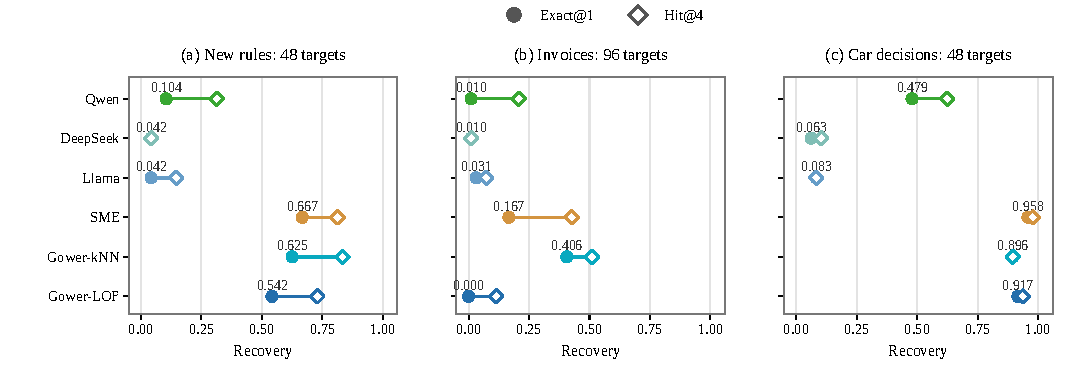
\includegraphics[width=\textwidth]{figures/figure_unified_transfer.pdf}
\caption{Unified support-localization configuration across three workloads. Filled circles show Exact@1 (annotated); open diamonds show Hit@4. New rules average 12 rule means, invoices four relation means, and Car decisions 48 targets from one source. SME is sample-minimal enumeration. All-query denominators and track-specific candidate caps are shared; these descriptive scores are not pooled.}
\label{fig:transfer}
\end{figure*}

Figure~\ref{fig:transfer} applies the same model configuration to the other support workloads. On 48 new-rule targets, Qwen/DeepSeek/Llama reach Exact@1 of 0.104/0.042/0.042. SME scores 0.667, compared with 0.625 for kNN and 0.542 for LOF. The largest truth-size stratum contains 16 targets with four- to six-field minima; complete strata and outcomes remain in the artifact. The original full-prompt Qwen score was 0.167, so the original result and the joint configuration are kept distinct.

On invoices, Qwen scores 0.010/0.208 at Exact@1/Hit@4; kNN scores 0.406/0.510, SME 0.167/0.427, and LOF 0.000/0.115. Eight invoice queries admit a four-field alternative, and five have only four-field minima, motivating the full 255-candidate search. Section VI investigates the LOF reversal on these fixed queries.

\textbf{Independent source with the same label semantics.} On Car decisions, SME obtains Exact@1/Hit@4 of 0.958/0.979; kNN and LOF obtain Exact@1 of 0.896 and 0.917. The model values are 0.479/0.063/0.083. This retains population-minimal support as the target, unlike corrected-cell or circuit transfer. The selected cohort contains 43 cases with a singleton minimum and 5 requiring multiple fields. On the latter subset, SME/Qwen/kNN/LOF reach 0.600/0.000/0.000/0.200. The predominance of simple exclusions and the single expert model limit conclusions about wider operational data.

\subsection{Repeated references and complete populations}
\begin{figure*}[t]
\centering
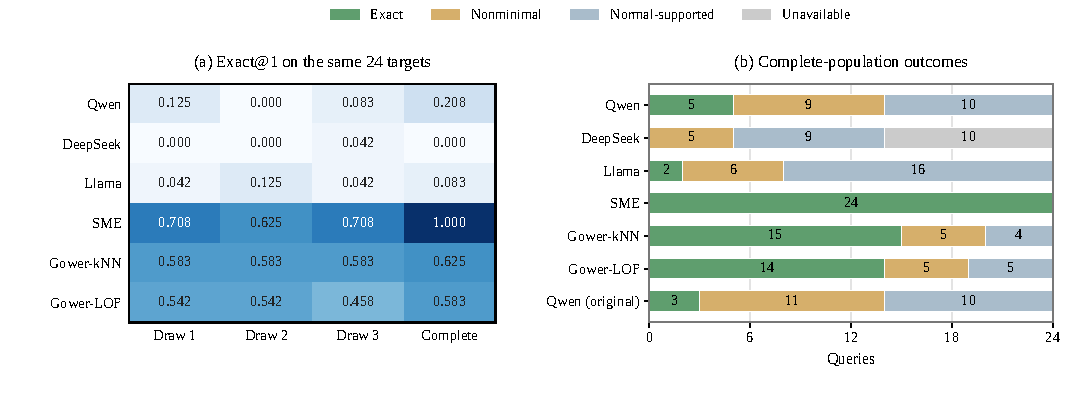
\includegraphics[width=\textwidth]{figures/figure_unified_evidence.pdf}
\caption{Evidence diagnosis on the same 24 targets from 12 new rules. (a) Exact@1 under three reference draws and complete normal evidence. (b) Complete-population error counts for the unified configuration; the last row retains original-prompt Qwen for comparison. Completeness also changes the prompt declaration. Sample-only exclusions are impossible in this condition.}
\label{fig:evidence}
\end{figure*}

SME exactly recovers valid minima on all 24 complete-population queries (Figure~\ref{fig:evidence}), as required by its search definition. The complete visible population therefore makes this finite task algorithmically solvable without hidden labels. Gower-kNN and LOF achieve Exact@1 of 0.625 and 0.583; their remaining errors show that a novelty-score ordering does not optimize minimal support directly. A full population removes sample absence ambiguity, but it does not make an arbitrary scoring function or generator exact.

The joint Qwen configuration reaches 0.208 under complete evidence, with 5 exact answers, 9 nonminimal exclusions, 10 supported sets, and 0 unavailable answers. The original full prompt produced three exact answers, 11 nonminimal exclusions, and 10 supported sets. These configurations must not be combined into one error partition. Their recorded errors show that missing references are not the only source of failure in the evaluated settings. Because completeness is also declared in the prompt, the comparison does not isolate a pure effect of adding rows.

Across the three finite draws, extra sample minima average 1.542/1.208/1.000 on the paired targets; complete evidence removes them. Figure~\ref{fig:evidence} reports every draw instead of selecting the most favorable sample. The artifact records first-set stability, candidate retention, and error types for each method. Stability and accuracy remain separate: a repeated wrong subset is stable, and a change between two valid minima need not be an error.

\subsection{How the output contract changes the comparison}
\begin{figure}[t]
\centering
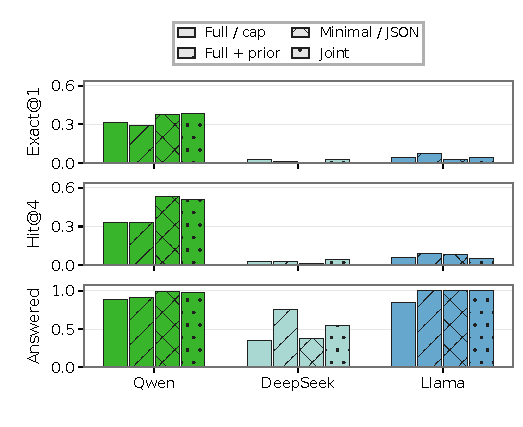
\includegraphics[width=\columnwidth]{figures/figure_unified_contract.pdf}
\caption{Configuration diagnostics on the same 96 targets. Full/cap applies the common size rule to original responses; Full+prior also states it. Minimal/JSON has constrained decoding without the three-field prior. Joint combines the core task, size information, and constrained output. Conditions differ as specified; connecting lines do not estimate individual factorial effects.}
\label{fig:contract}
\end{figure}

The original shared-prior experiment changes Qwen/DeepSeek/Llama Exact@1 from 0.313/0.031/0.042 to 0.292/0.010/0.073 under the same size-enforced scoring. No paired change passes its six-test Holm correction. This addresses that instruction within the original full contract; it cannot predict the joint configuration by itself.

The reduced unconstrained prompt produced 94 similarly malformed Qwen JSON objects among 95 actual generations, each missing a candidate-object closing brace, despite a valid example. None exhausted 512 output tokens. Fixed-schema decoding on that same minimal prompt raises Qwen Exact@1 from 0.000 to 0.375 and Hit@4 from 0.010 to 0.531. Llama's validity reaches 1.000 but its Exact@1 remains 0.031; DeepSeek's nine output-cap failures and abstentions still limit usable answers. The joint configuration in Table~\ref{tab:unified} incorporates reliable output structure and shared size information in the same run.

The original non-answer bound, $\mathrm{Exact@1}+1-\mathrm{Answered}$, gives 0.239/0.292/0.211 for Qwen/DeepSeek/Llama, below LOF's original 0.514. This calculation holds existing answers fixed. It cannot bound an intervention that changes the content of already answered queries, as the contract experiments demonstrate.

\subsection{Original suite and adapter behavior}
\begin{table}[t]
\centering\footnotesize
\caption{Original 864-case diagnostic: mean $\pm$ SD across 38 templates. Gower and SME use a three-field prior absent from the original LLM prompt. Rule, size and behavior metrics remain in the artifact; this is not the unified primary comparison.}
\setlength{\tabcolsep}{3pt}
\renewcommand{\arraystretch}{1.12}
\begin{tabular}{lrrr}
\toprule
Method & Exact@1 & Hit@4 & Suff.@1 \\
\midrule
Qwen (original) & $0.231\!\pm\!0.215$ & $0.249\!\pm\!0.210$ & $0.537\!\pm\!0.300$ \\
DeepSeek (original) & $0.023\!\pm\!0.037$ & $0.039\!\pm\!0.051$ & $0.291\!\pm\!0.145$ \\
Llama (original) & $0.032\!\pm\!0.043$ & $0.049\!\pm\!0.059$ & $0.183\!\pm\!0.161$ \\
Gower-LOF & $0.514\!\pm\!0.360$ & $0.637\!\pm\!0.328$ & $0.538\!\pm\!0.366$ \\
Gower-kNN & $0.411\!\pm\!0.302$ & $0.499\!\pm\!0.284$ & $0.608\!\pm\!0.330$ \\
SME & $0.232\!\pm\!0.218$ & $0.549\!\pm\!0.359$ & $0.232\!\pm\!0.218$ \\
RLAX adaptation & $0.426\!\pm\!0.384$ & $0.478\!\pm\!0.367$ & $0.498\!\pm\!0.407$ \\
SOD adaptation & $0.000\!\pm\!0.000$ & $0.000\!\pm\!0.000$ & $0.610\!\pm\!0.438$ \\
COP adaptation & $0.011\!\pm\!0.028$ & $0.021\!\pm\!0.035$ & $0.011\!\pm\!0.028$ \\
Univariate top four & $0.144\!\pm\!0.207$ & $0.391\!\pm\!0.406$ & $0.144\!\pm\!0.207$ \\
Random size & $0.033\!\pm\!0.021$ & $0.123\!\pm\!0.076$ & $0.108\!\pm\!0.084$ \\
All fields & $0.000\!\pm\!0.000$ & $0.000\!\pm\!0.000$ & $1.000\!\pm\!0.000$ \\
First three & $0.002\!\pm\!0.014$ & $0.002\!\pm\!0.014$ & $0.220\!\pm\!0.139$ \\
\bottomrule
\end{tabular}
\renewcommand{\arraystretch}{1.0}
\label{tab:original}
\end{table}

The secondary original comparison illustrates why sufficiency alone is inadequate. Qwen and LOF have Suff@1 of 0.537 and 0.538, but Exact@1 of 0.231 and 0.514; no equivalence is claimed. SOD's Suff@1 is 0.610 with zero exact recovery and a mean selected-field fraction of 0.577. The expanded suite is useful for characterizing objectives, while the unequal original prior prevents treating it as the unified primary ranking.

Native controls help interpret low adapted scores. On M\textsuperscript{2}OE's continuous repository example, 30 epochs recover the three injected fields in 7 of 10 seeds, with mean choice precision/recall 1.000/0.900. Returned patches reduce distance outside the unit cube by 0.827 on average. At 300 epochs, exact recovery is zero, recall 0.600, and distance reduction 0.375. SOD includes all three shifted low-variance coordinates in all 20 native cases, but selects extra fields and has mean precision 0.389. These checks demonstrate native behavior without validating the mixed-type minimum-support adaptation or establishing convergence.

Original sensitivity diagnostics also remain informative. Across four random displays of the paired panel, Qwen's Exact@1 spans 0.240--0.313 and its conditional top-one agreement is 0.256; Gower rankings are invariant to display order. Nested 8/16/32 references yield population-minimum retention 0.703/0.849/0.911 and original Qwen Hit@4 of 0.177/0.250/0.333. Expanding all 288 six-field cases from 41 bounded candidates to all 63 changes LOF Exact@1 from 0.550 to 0.544 and kNN from 0.467 to 0.442. Exhaustive effects at 12/24 fields remain unmeasured. These diagnostics characterize their original configurations and do not substitute for the new joint comparisons.

\section{Why Subspace Scores Reverse Across Workloads}
\subsection{RQ3: Candidate space and neighborhood size}
LOF leads the original support comparison but reaches zero exact recovery on the invoices. The unified configuration leaves its statistical predictions unchanged. Restricting the same invoice search from eight fields to three leaves Exact@1 at 0.000; every winning original LOF set already has at most three fields. kNN instead changes from 0.406 to 0.438. Thus, the larger maximum candidate size does not explain the zero LOF score through larger winning sets.

At $k=1/3/5/10$, invoice LOF Exact@1 is 0.021/0.000/0.063/0.021, compared with kNN's 0.240/0.406/0.396/0.292. The reversal persists across these neighborhood sizes. Every original LOF winner has a target neighbor whose mean reachability distance falls below the $10^{-9}$ floor; 88 of 96 winning sets contain a distractor. This motivates inspecting local densities and the competition between projections.

\subsection{From duplicate projections to candidate order}
Breunig et al.~\cite{breunig2000lof} already identify infinite local reachability density caused by duplicate points and discuss neighborhoods based on distinct coordinates. Their $k$-distance neighborhood also includes all boundary ties. Our additional question is how duplicate structures created by \emph{projection}, numerical floors, and competition among candidate subspaces affect retrieval of population-minimal explanations. Duplicate-induced density degeneracy itself is not a new finding.

For the original fixed-$k$ adapter, let $N_k(u)$ be the selected reference neighbors and $d_k(v)$ the reference $k$-distance in subspace $S$. It computes
\begin{align}
a_S(u)&=k^{-1}\sum_{v\in N_k(u)}\max\{d_S(u,v),d_k(v)\},\\
\ell_S(u)&=1/\max\{a_S(u),\epsilon\},\\
\mathrm{LOF}_S(x^*)&=\frac{k^{-1}\sum_{v\in N_k(x^*)}\ell_S(v)}{\ell_S(x^*)}.
\end{align}
Reference neighborhoods exclude the row itself. The extra denominator floor in the implementation is inactive here because Gower distances are bounded. A duplicate group can set a neighbor's density to $1/\epsilon$, while other target neighbors keep the target's own mean reachability positive. The resulting ratio can be large even when a reference exactly matches the target projection. Support depends on whether a match exists; this density ratio also depends on multiplicities and nearby distances.

For \texttt{constraint\_line\_net\_000}, supported distractor pair \{F002,F003\} scores $1.67\times10^8$, while the highest-ranked valid minimum \{F001,F004,F008\} scores 3.033. In the motivating tax case, supported singleton F005 scores $3.33\times10^8$, above valid pair \{F004,F008\} at $2.89\times10^8$. Searching all projections compares scores with different duplicate structures and scales. These traces identify a mechanism in this adapter; they do not establish that arithmetic anomalies generally defeat LOF.

\begin{figure*}[t]
\centering
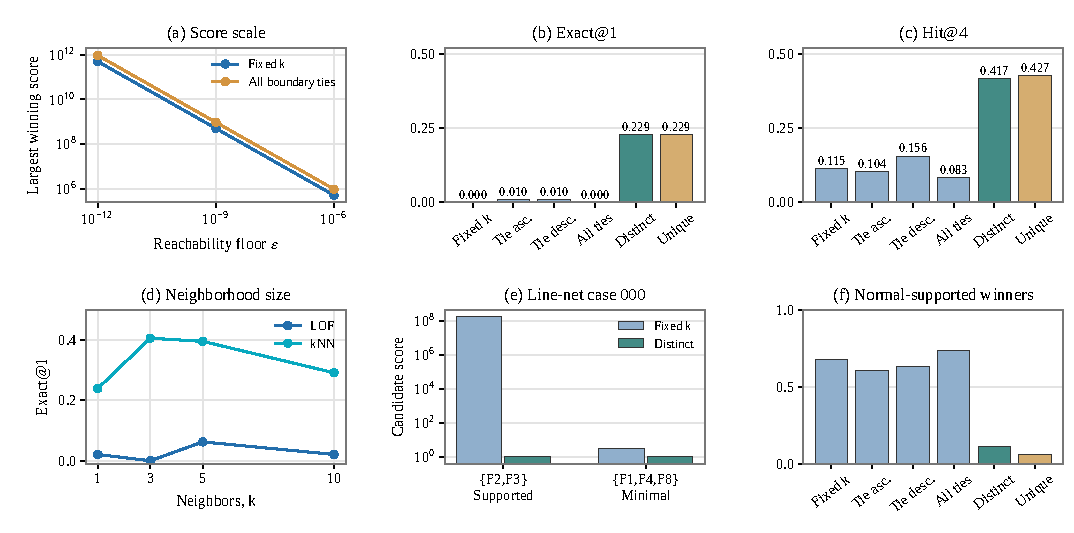
\includegraphics[width=\textwidth]{figures/figure_unified_lof.pdf}
\caption{Matched invoice LOF diagnostics, all 96 targets and 255 candidates. (a) The floor changes score scale. (b)--(c) Recovery under fixed-$k$ tie choices, all boundary ties, distinct-coordinate radii retaining multiplicities, and unique projections. (d) Original neighbor-count sweep. (e) Supported and valid-minimal candidates in line-net case 000. (f) Fraction of winners already supported by a normal reference. Recovery panels use equal-relation means; variants retain their stated neighborhood semantics.}
\label{fig:lof}
\end{figure*}

\subsection{Floor, ties, and duplicate-aware variants}
\textbf{Numerical floor.} With the original neighbor routine, changing $\epsilon$ from $10^{-6}$ through $10^{-9}$ to $10^{-12}$ changes score magnitudes by approximately six orders but leaves all first choices unchanged. Exact@1 remains 0.000 and Hit@4 0.115. Inclusive-boundary neighborhoods likewise retain Exact@1 0.000 and Hit@4 0.083 throughout the sweep. The large score scale is floor-dependent; the observed failure is not removed by these floor choices.

\textbf{Boundary ties.} Canonical ascending and descending fixed-$k$ tie choices change 58 and 54 of 96 first sets relative to the original routine. Both reach Exact@1 0.010; their Hit@4 values are 0.104 and 0.156. Including every $k$-distance boundary tie changes 54 first choices, but exact recovery remains zero. Thus, discrete ties materially affect which explanations are returned, while boundary inclusion alone does not resolve this reversal. The original fixed-$k$ implementation must remain distinguished from the original LOF neighborhood definition.

\textbf{Duplicate treatment.} A distinct-coordinate radius retaining reference multiplicities reaches Exact@1/Hit@4 of 0.229/0.417. Collapsing identical projections and using inclusive boundaries reaches 0.229/0.427. Their fractions of normal-supported winners fall to 0.115 and 0.063, versus 0.677 for the original routine. The variants change neighborhood semantics, and projection collapse also changes empirical weights. Both improve recovery but remain below kNN's Exact@1 0.406 on this workload.

Earlier diagnostic restrictions remain separate: hidden-role-only search reaches LOF Exact@1 0.219; fixed-$k$ projection deduplication and exploratory reference-percentile calibration each reach 0.240. The oracle restriction uses hidden information, and reference-percentile scores share the fitted graph rather than an independent calibration sample. Their purpose is explanation of the original ranking, not selection of the best variant after observing test results. Taken together, the interventions locate the additional phenomenon in cross-projection competition among duplicate-sensitive scores.

\section{External Targets and Practical Scope}
\subsection{Public corrected-field inspection}
\begin{figure}[t]
\centering
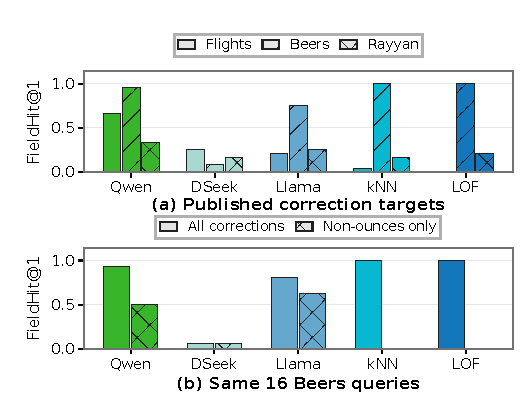
\includegraphics[width=\columnwidth]{figures/figure_unified_corrections.pdf}
\caption{Structured singleton inspection on published corrections. (a) Each source contains 24 targets. (b) The same 16 Beers queries with non-ounces corrections are evaluated against all recorded changes and then only non-ounces changes, with predictions fixed. These endpoints assess correction localization, not population-minimal support.}
\label{fig:corrections}
\end{figure}

The public-correction results concern a different task. Fixed structured decoding raises Qwen's equal-source FieldHit@1 from 0.125 to 0.653, and Llama's from 0.056 to 0.403; both Gower controls score 0.403. Qwen covers 0.721 of recorded corrections within three suggestions. Its mean first-correction inspection score is 2.819, compared with kNN's 3.681 and an analytic uniform ordering's 4.253 under the same cap and failure penalty. These are offline ranking quantities, not measurements of analyst time.

\textbf{Correction type matters.} All 24 Beers targets contain an ounces representation change, and both Gower methods choose a corrected field first in every case. Our source audit identifies 24 quantity representations, 12 missing-marker normalizations, six city/state split changes, and seven percentage conventions. Seventeen rows contain only the explicitly checked row-local normalizations; seven mix them with percentage interpretation. Removing ounces from the accepted fields on the same 16 multi-correction queries reduces Gower FieldHit@1 to 0.000. Qwen and Llama retain 0.500 and 0.625; Gower Hit@3 remains 0.750. The first-choice result therefore depends strongly on the repeated ounces pattern, while later candidates retain useful coverage.

Flights contains 28 changed clock values and 21 imputations, alongside three clock-preserving format changes. The references exclude the query's flight; an actual-departure correction such as 11:06 to 11:05 requires event-specific evidence unavailable in other flights. Qwen's FieldHit@1 of 0.667 indicates selection of a recorded changed field, not recovery of that external fact. Rayyan contains date serialization, encoding normalization, missing sentinels, and other bibliographic conventions. The audit preserves those supplied labels without claiming an independent judgment that each canonical value is semantically correct. Neither source-convention agreement nor model consensus certifies a minimal explanation.

\subsection{Auxiliary pilots and interpretation}
The peer pilot retains 390 model outputs, including 349 valid non-abstentions. Pairwise Jaccard ranges from 0.213 to 0.520 on 40 ADBench queries answered by all five models; UCI has only one common-valid query. The archived Pima example has Qwen/peer-majority overlap 0.500, with no field-level truth. These measurements characterize agreement only.

With all circuit outputs visible, Qwen/DeepSeek/Llama achieve Jaccard@4 of 0.349/0.109/0.038, compared with input-only Gower-kNN/LOF at 0.456/0.428. Qwen's Hit@4 is 0.016 and the others retrieve no exact fault set. Scores average queries within targets, targets within table pairs, and pairs within four circuits. These fault labels and the limited number of circuits prevent treating the pilot as validation of population-minimal support.

\textbf{Method selection.} First specify the accepted object: an irreducible unusual combination, a rule mechanism, or a field recorded as corrected. Under the support objective, inspect both candidate coverage and rank: SME can expose useful alternatives while placing a spurious small set first. For density-based search, inspect projection duplicates, boundary ties, and score magnitudes. For LLMs, the prompt, candidate information, decoder, parser, and abstention rule together define the compared method. The unified results and the invoice diagnostics support these choices within the measured workloads; they do not yield one ranking across all label types.

\textbf{Continuous and noisy data.} For independently sampled continuous values, an exact match to a new normal value almost surely does not occur in a finite reference sample. Applying literal sample absence would then make ordinary singletons appear explanatory. Extending this benchmark requires a specified support model or explicit scales, tolerance neighborhoods, and a mass threshold, which change the gold labels. The integer invoice constraints and finite expert decision table avoid that ambiguity. Native continuous adapter checks do not validate a continuous version of the support benchmark.

\section{Related Work}
\textbf{Closest evaluation predecessor.} Myrtakis et al.~\cite{myrtakis2021comparative} compare relevant-subspace explanation algorithms using multiple ground-truth subspaces and exact membership for Recall/MAP. Their synthetic evaluation includes cases where lower-dimensional projections mix outliers with normal points. We build on that evaluation setting rather than claim multiple answers or exact matching as new. Our increment is complete enumeration of population-minimal support families, an explicit finite-reference interface, and separate rule/edit labels. These distinctions enable audits of extra sample minima and label-dependent scores. Beam permits varying dimensions; RefOut fixes dimensionality. Our Beam adaptation is accompanied by a size-matched exhaustive control.

\begin{table}[t]
\centering\footnotesize
\caption{Direct relationship to neighboring evaluation targets. Entries describe the evaluated object, not exhaustive software capabilities.}
\setlength{\tabcolsep}{3pt}
\begin{tabularx}{\columnwidth}{lXX}
\toprule
Work & Evaluation target & Relation to this study \\
\midrule
Myrtakis et al.~\cite{myrtakis2021comparative} & Relevant subspaces; multiple labels, exact match & We enumerate full population minima and audit finite evidence \\
M\textsuperscript{2}OE~\cite{angiulli2024m2oe} & Field choices and repairs & Repair fields and minimal support are separated \\
Circuit labels~\cite{antwarg2024groundtruth} & Fault-related input sets & Auxiliary fault target, not support truth \\
Raha/Baran~\cite{mahdavi2019raha,mahdavi2020baran} & Detection/correction of dirty cells & Published changes provide inspection targets \\
\bottomrule
\end{tabularx}
\label{tab:closest}
\end{table}

\textbf{Explanation objectives.} Surveys distinguish instance descriptions from detector-score explanations~\cite{panjei2022survey,li2024xadsurvey}. Shapley-style explanations and CAIT attribute model behavior~\cite{kluttermann2024shapley,mok2025cait}; LookOut, SOD, COP, and RLAX select or rank subspaces~\cite{gupta2018lookout,kriegel2009sod,kriegel2012cop,amirato2026rlax}. M\textsuperscript{2}OE also optimizes repair information~\cite{angiulli2024m2oe}. Aggregate diagnosis systems such as Scorpion, Adtributor, iDice, HotSpot, and Squeeze explain changes in aggregate behavior~\cite{wu2013scorpion,bhagwan2014adtributor,lin2016idice,sun2018hotspot,li2019squeeze}. These objectives need not identify the same fields as support minimality.

\textbf{Data quality and recent ICDE systems.} HoloClean, holistic repair, and AutoDCWorkflow address cleaning workflows and integrity errors~\cite{rekatsinas2017holoclean,chu2013holistic,li2025autodcworkflow}. BClean uses Bayesian networks and user priors~\cite{qin2024bclean}; ZeroED and ZeroEC use LLMs for error detection and context-informed correction~\cite{ni2025zeroed,wu2025zeroec}. Query verification and AutoTest study additional data-quality operations~\cite{schreiber2026verification,chen2025autotest}. These systems motivate the application, while the present task deliberately withholds the clean target and evaluates combinations rather than a unique repair value.

\textbf{Benchmarks and component analysis.} ADBench supplies anomaly benchmarks~\cite{han2022adbench}; TABARD, RADAR, AnTBench, and SEC-FinTables evaluate perturbed tables, anomaly reasoning, awareness, or financial inconsistencies~\cite{choudhury2025tabard,gu2025radar,wei2026antbench,ke2026secfintables}. Papadakis et al.~\cite{papadakis2024reevaluation} show why candidate construction matters in record linkage. Recent ICDE EAB studies decompose retrieval and generation, table-retrieval design, counting methods, and adaptive-query-processing components~\cite{zhang2026xrag,yang2026tr360,zhu2026beacon,mu2026aqp}. Our analogous methodological goal is to identify which evidence, output, and scoring conditions produce the observed explanation rankings.

\section{Artifact and Reproducibility}
The public repository at \url{https://github.com/KDDElab/known-outlier-benchmark} and its fixed \href{https://github.com/KDDElab/known-outlier-benchmark/releases/tag/icde2027-eab-v3}{\texttt{icde2027-eab-v3}} release provide generators, frozen inputs and population labels, raw responses, baseline outputs, analysis, figures, manuscript sources, dependencies, and file hashes. Inspecting predictions and recomputing scores require no private inference service. UCI Car Evaluation is attributed under CC BY 4.0; existing correction and circuit sources retain their provenance and licenses.

The new unified archive contains 1,080 model-query records, 1,080 statistical/enumeration predictions, and 14 LOF diagnostic conditions with candidate scores. It preserves the original 5,184 model-condition records, 288 invoice responses, and 1,368 earlier revision records separately. IDs and manifests prevent counting provenance copies as extra cases. The population-label mapping of the new-rule source is explicit: its sample-reference minima remain diagnostic, while complete-population labels are independently reconstructed from its normal table.

Inference uses Transformers 5.22.1, PyTorch 2.14.1+cu126, bf16, RTX 3090 GPUs, and batch size one. Model and tokenizer fingerprints, chat templates, input hashes, greedy settings, LM Format Enforcer 0.11.3, and its compatibility shim are recorded. Weights are obtained from the documented upstream providers under their access terms. Different GPU allocations and tokenizers preclude a controlled cost or speed ranking.

README commands rebuild analyses and the PDF from frozen outputs. Changed-path checks independently verify 168 new-rule/Car population label sets, reproduce 624 existing Gower candidate lists, and compare 552 inclusive-neighborhood scores with a scalar implementation. Complete-population SME outputs match the independently enumerated gold families. Packaged reconstruction is performed on the original host; independent-machine and bitwise fresh-inference reproduction remain unverified.

\section{Limitations}
\textbf{Coverage and independence.} The original templates overlap between development and test across seeds, and earlier results informed later evaluation choices. Twelve new compositions provide a small Boolean workload; the current joint protocol reuses those already examined queries. Car adds an independently published decision model with targets selected before joint inference, but it is one finite expert system with many singleton exclusions. Four invoice relations and four circuits do not establish broad operational coverage. Temporal anomalies and MAR/MNAR missingness remain untested.

\textbf{Methods and evidence.} The results concern three local checkpoints and fixed prompts, not the capability frontier of LLMs. Development checks do not prove adapter convergence. Three reference draws and 24 complete-population targets do not identify a universal lower bound on error; completeness jointly changes coverage and the prompt declaration. Support--rule discrepancies concentrate in deterministic proxies, and exact finite-domain support does not directly extend to continuous noise.

\textbf{External meaning.} Published corrections include canonicalization and source conventions; agreement with them is not an independently adjudicated minimal explanation. The source audit adds no human judgments, disagreement records, or observed time-saving measurements. The independent expert table preserves the core label semantics but does not supply natural anomaly incidents. Pretraining exposure cannot be excluded by opaque identifiers, and fresh inference remains sensitive to software, kernels, and checkpoint access.

\section{Conclusion}
Anomaly-explanation evaluation depends on the object being recovered. Complete population-minimal labels expose differences from rule mechanisms and edit histories; finite references introduce additional plausible sets. The unified comparison jointly controls candidate information and output structure, while direct sample enumeration separates candidate coverage from ranking. Complete populations make the finite task solvable but do not make every tested generator or score exact. Invoice diagnostics connect a ranking reversal to duplicate structures, neighbor selection, and cross-subspace density competition, with effects that persist under several numerical choices. These findings support configuration-specific method comparisons and keep correction localization, fault recovery, and peer agreement distinct from minimal support explanation.

\label{page:main-end}
\clearpage
\section*{Acknowledgments and AI Use Disclosure}
OpenAI Codex assisted with English drafting throughout the manuscript, benchmark code and experiments in Sections III--VII, and Figures 1--7 and tables. The author is responsible for verifying the archived measurements, claims, citations, and code.
\bibliographystyle{IEEEtran}
\bibliography{phase_d_references}
\end{document}
